\documentclass[10pt]{acmtrans2e}
\usepackage{hyperref}
\usepackage{amsmath}
\usepackage{amssymb}
\usepackage{amsfonts}
\usepackage{amscd}
\usepackage{amsmath}
\usepackage{latexsym}
\usepackage{graphicx}
\usepackage{geometry}
\usepackage{tikz-uml}
\usepackage{ifthen}
\usepackage{multicol}
\usepackage{paralist} % for compactitem und compactenum
% \usepackage{ellipsis}
\frenchspacing
\usepackage{nth}     % oridinal numbers: 1st, 2nd, ... by \nth{1}, \nth{2}, ...
                     % \usepackage[super]{nth} % Option 'super' not available at University
\usepackage{xspace}
\usepackage{enumitem}
\usepackage{listings}
\usepackage{epstopdf}

\hypersetup{
  colorlinks = false,
  urlcolor = blue,
  linkcolor = blue,
  pdfauthor = {Hao Lin},
  pdfkeywords = {Consensus clustering, $K$-means, utility function, MATLAB},
  pdftitle = {User Manual for KCC---a MATLAB package for K-means-based Consensus Clustering},
  pdfsubject = {KCC package},
  pdfpagemode = UseNone
}

\geometry{
  left=4cm,
  right=4cm,
  top=4cm,
  bottom=4cm
}

\newcommand{\Matlab}{\textsc{Matlab}}
\newcommand{\Octave}{\textsc{Octave}}
\newcommand{\KCC}{\textsf{KCC}\xspace} % package's name: \textsf{tboxIPscatt} and dynamic space

\newlength{\tabcont}
\newcommand{\tab}[1]{%
\settowidth{\tabcont}{#1}%
\ifthenelse{\lengthtest{\tabcont < 1cm}}%
{\makebox[1cm][l]{#1}\ignorespaces}%
{\makebox[2cm][l]{#1}\ignorespaces}%
}%

\newcommand{\syntax}[1]{\medskip
\noindent \textbf{Syntax:} \medskip

\texttt{#1}
}

\newenvironment{inputlist}
{\vspace*{0.25cm}
\noindent \textbf{Input parameters:}
\begin{itemize}
}  
{ 
\end{itemize}
}

\newenvironment{outputlist}
{\vspace*{0.075cm}
\noindent \textbf{Output parameters:}
\begin{itemize}
}  
{ 
\end{itemize}
}

\newenvironment{remark}
{\vspace*{0.1cm}
\noindent \textbf{Discussion:} \medskip

}
{
\vspace*{0.2cm}
}

\newenvironment{example}
{\vspace*{0.1cm}
\noindent \textbf{Example:} \vspace*{0.15cm}

\setlength{\parskip}{0.5ex plus 0.5exminus 0.2 ex}
}
{\medskip
}

\newcommand{\paramitem}[2]{\item[] \tab{\texttt{#1}} \tab{: #2} }

\firstfoot{}
\runningfoot{}

\markboth{Hao Lin}{User Manual for \KCC---a {MATLAB} package for K-means-based Consensus Clustering}

\title{User Manual for \KCC---a {MATLAB} package for K-means-based Consensus Clustering} 

% \author{Hao Lin}
% \orcid{0000-0002-1921-3036}
% \email{linh@in.tum.de}
% \affiliation{%
%   \institution{Department of Informatics, Technical University of Munich}
%   \streetaddress{Boltzmannstr. 3}
%   \city{Garching}
%   \postcode{85748}
%   \country{Germany}
% }

% \author{Hongfu Liu}
% \email{hongfuliu@brandeis.edu}
% \affiliation{%
%   \institution{Michtom School of Computer Science, Brandeis University}
%   \streetaddress{415 South St}
%   \city{Waltham}
%   \state{MA}
%   \postcode{02453}
%   \country{USA}
% }

% \author{Junjie Wu}
% \authornote{Corresponding Author}
% \email{wujj@buaa.edu.cn}
% \affiliation{%
%   \institution{School of Economics and Management, Beihang University}
%   \streetaddress{37 Xueyuan Rd}
%   \city{Haidian District}
%   \state{Beijing}
%   \postcode{100191}
%   \country{China}
% }

% \author{Hong Li}
% \email{hong_lee@buaa.edu.cn}
% \affiliation{%
%   \institution{School of Economics and Management, Beihang University}
%   \streetaddress{37 Xueyuan Rd}
%   \city{Haidian District}
%   \state{Beijing}
%   \postcode{100191}
%   \country{China}
% }

% \author{Stephan Günnemann}
% \email{guennemann@in.tum.de}
% \affiliation{%
%   \institution{Department of Informatics, Technical University of Munich}
%   \streetaddress{Boltzmannstr. 3}
%   \city{Garching}
%   \postcode{85748}
%   \country{Germany}
% }

\author{
Hao Lin\footnote{Department of Informatics, Technical University of Munich, Germany,
\textsf{\href{mailto:linh@in.tum.de}{linh@in.tum.de}}.}, \quad
Hongfu Liu\footnote{Michtom School of Computer Science, Brandeis University, USA, \textsf{\href{mailto:hongfuliu@brandeis.edu}{hongfuliu@brandeis.edu}}.}, \quad
Junjie Wu\footnote{School of Economics and Management, Beihang University, China, \textsf{\href{mailto:wujj@buaa.edu.cn}{wujj@buaa.edu.cn}}.}, \quad
Hong Li\footnote{School of Economics and Management, Beihang University, China, \textsf{\href{mailto:hong_lee@buaa.edu.cn}{hong\_lee@buaa.edu.cn}}.}, \quad
Stephan Günnemann\footnote{Department of Informatics, Technical University of Munich, Germany, \textsf{\href{mailto:guennemann@in.tum.de}{guennemann@in.tum.de}}.}
}
\date{User Manual for \KCC, updated \today}

\begin{document}

\maketitle

\vspace*{-0.5cm}

\section{Introduction}

This user manual systematically presents the usage of the \Matlab{} package on K-means-based Consensus Clustering (KCC) accompanying the following paper:
\begin{center}
\begin{minipage}{0.90\textwidth}
Hao Lin, Hongfu Liu, Junjie Wu, Hong Li, and Stephan Günnemann. 2022. Algorithm xxxx: KCC: A MATLAB Package for K-means-based Consensus Clustering. \emph{ACM Trans. Math. Softw}.
\end{minipage}
\end{center}

\noindent The package was developed and tested in \Matlab{} R2012a under Linux. {\color{red}To those without access to \Matlab{} and those who prefer to use free open source software, we also investigate the usage of \KCC with \Octave{}, and find it is also compatible with \Octave{} without additional efforts. \Octave{} version?}. 

For package installation, you need to first unpack the compressed archive into your current directory. It consists of a \emph{source code} folder \textsf{Matlab}, a folder \textsf{userManual} with this comprehensive \emph{user manual}, and a \emph{license} file \textsf{LICENSE} indicating that the package is distributed under GNU GENERAL PUBLIC LICENSE (Version 3). Then under the \textsf{Matlab} folder, you need to add one of its subfolder, i.e., the \textsf{Src} folder, to the \Matlab{} path. The directory structure of the \textsf{Matlab} folder is described as follows.
% All computations in this \emph{user guide} were carried out on a workstation with an Intel(R) Core(TM) i7-3770 CPU with 3.40\,GHz and 32\,GByte RAM. For the given code snippets we recommend more than 5\,GByte RAM. This, in particular, is true for the three-dimensional reconstruction example as it is the most RAM-consuming one.
% It can be downloaded from the ACM Collected Algorithms (CALGO). 

% \setlength{\columnseprule}{0.25pt}
% \setlength{\columnsep}{10pt}
% \begin{multicols}{2}[][10mm]
\begin{compactitem}
  \item \textsf{Src} (core functions for conducting KCC)
  \begin{compactitem}
   \item \textsf{BasicCluster\_RFS.m} (function to generate BPs with RFS)
   \item \textsf{BasicCluster\_RPS.m} (function to generate BPs with RPS)
   \item \textsf{Preprocess.m} (function to prepare for consensus clustering)
   \item \textsf{KCC.m} (consensus function)
   \item \textsf{exMeasure.m} (function to compute validity scores for clustering results)

   \item \textsf{load\_sparse.m} (auxiliary function to load input text data as a sparse matrix)
   \item \textsf{hungarian.m} (auxiliary function for cluster label assignment)
   \item \textsf{BasicCluster\_RPS\_missing.m} (auxiliary function to generate IBPs with strategy-I)
   \item \textsf{addmissing.m} (auxiliary function to generate IBPs using strategy-II)
   \item \textsf{distance\_*} (distance functions)
   \item \textsf{gClusterDistribution.m} (auxiliary function to calculate cluster distribution for BPs)
   \item \textsf{Ucompute.m, Ucompute\_miss.m} (auxiliary function for utility calculation)
   \item \textsf{gCentroid.m, gCentroid\_miss.m} (auxiliary function for centroid update)
   \item \textsf{sCentroid.m, sCentroid\_miss.m} (auxiliary function for centroid initialization)
  \end{compactitem}
  \item \textsf{Drivers} (illustrative examples)
  \begin{compactitem}
   \item \textsf{data} (input data for illustration)
   \item \textsf{demo.m} (function for KCC with different utility functions)
   \item \textsf{demoIBPI.m} (function for KCC with IBPs generated by strategy-I)
   \item \textsf{demoIBPII.m} (function for KCC with IBPs generated by strategy-II)
   \item \textsf{demoNumberBP.m} (function for KCC with varying number of BPs)
   \item \textsf{demoStrategyBP.m} (function for KCC with RFS strategy for BP generation)
  \end{compactitem}
\end{compactitem}
% \end{multicols}

\begin{figure*}[!bt]
\centering
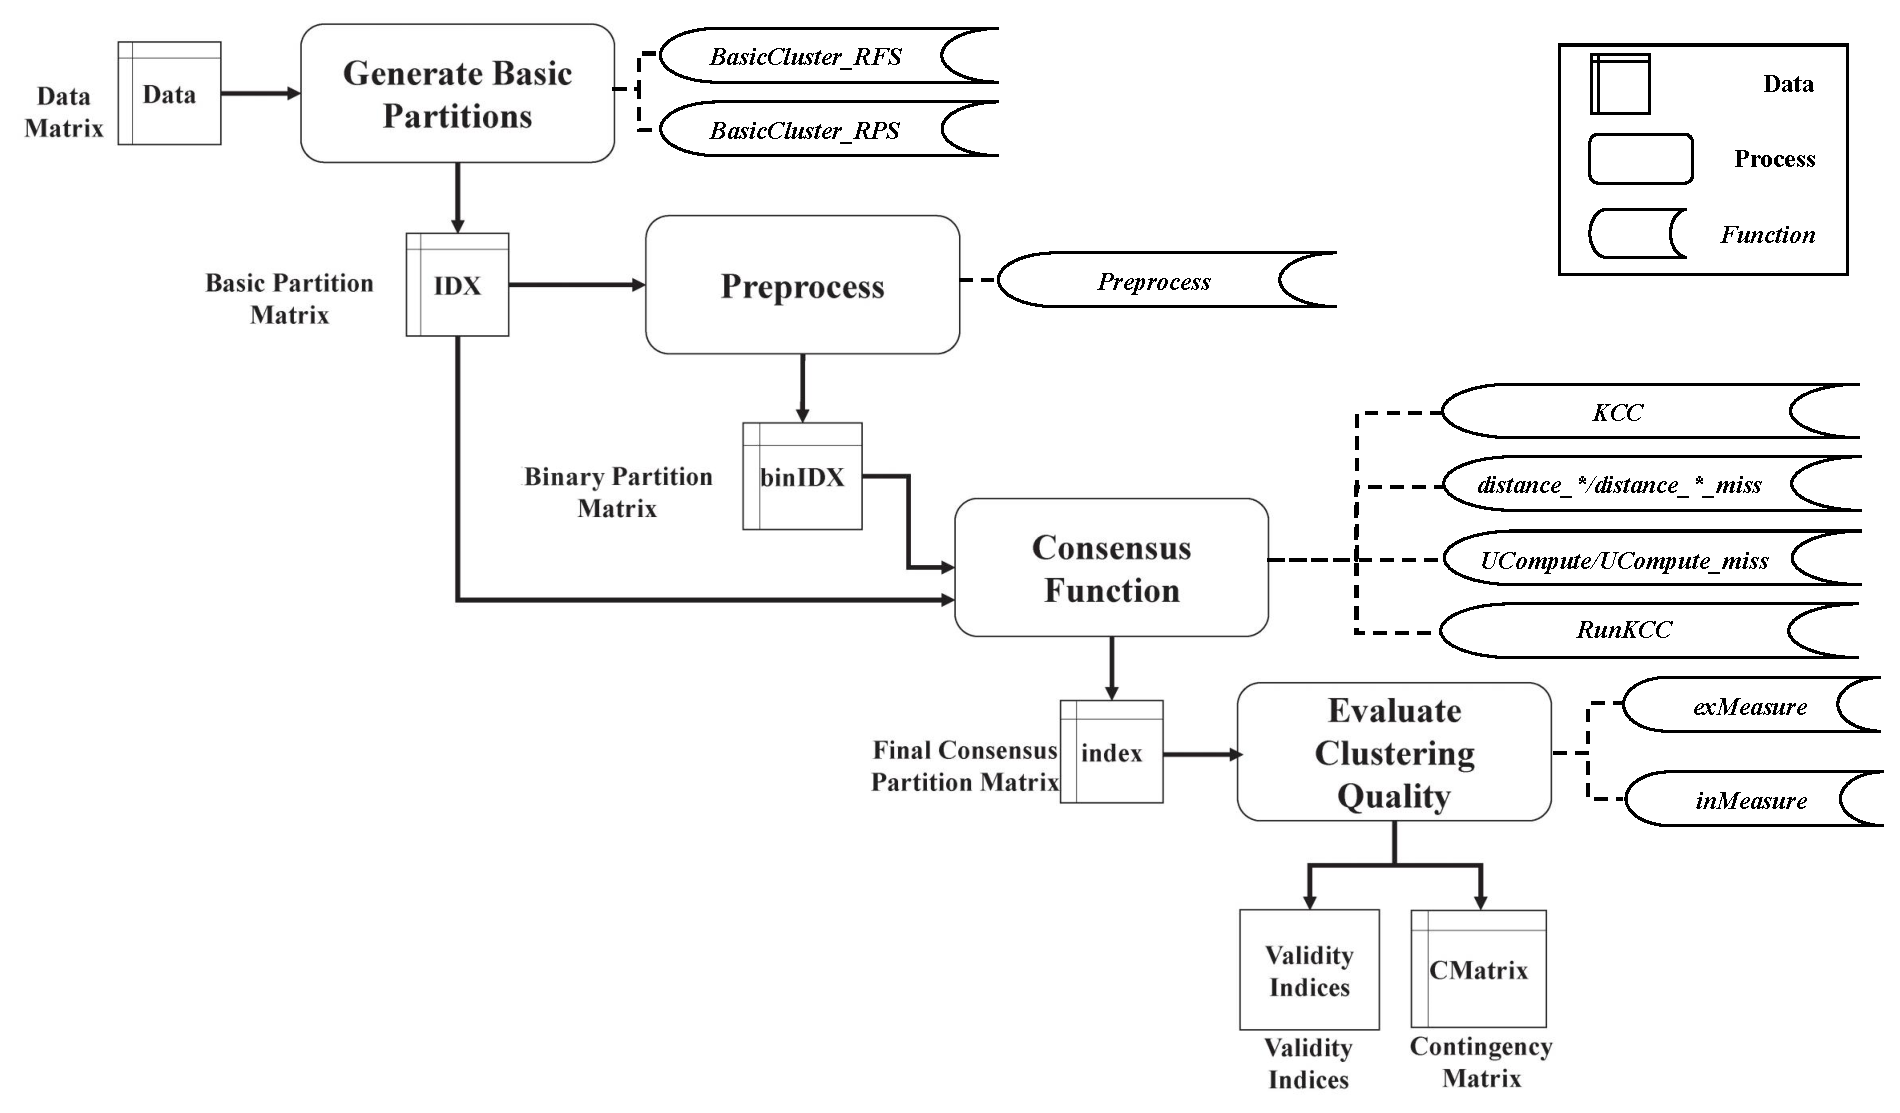
\includegraphics[width=0.85\textwidth]{fig/soft.eps}
\caption{Typical program flow of \KCC package.}\label{fig:soft} % \label should be placed after \caption
\end{figure*}

Figure~\ref{fig:soft} illustrates a typical program flow of using the \KCC package, which includes data preparation, basic partitions generation, consensus clustering preprocessing, consensus function, and clustering quality evaluation. We can see from Figure~\ref{fig:soft} that, in a typical flow for consensus clustering, a real-world matrix \textsf{Data} is first input to generate a basic partition matrix \textsf{IDX}. The basic partition matrix is then input to a \textsf{Preprocess} function to produce the sparse representation of $\mathcal{X}^{(b)}$, i.e., the binary matrix \textsf{binIDX}. The binary matrix \textsf{binIDX}, along with the basic partition matrix \textsf{IDX} is the input of the final consensus clustering via a $K$-means heuristic, also known as consensus function, which produces a consensus partition matrix \textsf{index}. Lastly, the clustering quality is evaluated with an \textsf{exMeasure} function, which outputs several external validity indices and a contingency matrix. We will take a detailed look at the important functions and fields in the Guides in Section~\ref{sec:guides}.

\section{Guides}\label{sec:guides}

\syntax{IDX = BasicCluster\_RFS(Data,r,K,dist,nFeature}

\begin{inputlist}
  \paramitem{Data}{an \textsf{n} $\times$ \textsf{p} matrix of data, whose rows correspond to \textsf{n} observations, and columns correspond to \textsf{p} features}
  \paramitem{r}{  }
  \paramitem{K}{  }
  \paramitem{dist}{\textsf{sqEuclidean} namely the squared Euclidean distance, and each centroid is the mean of the data points in a cluster}
  \paramitem{nFeature}{sampled uniformly at random without replacement from the integers \textsf{1} to \textsf{p}, which forms the indices of the selected features}
\end{inputlist}

\begin{outputlist}
  \paramitem{IDX}{a \textsf{n} $\times$ \textsf{r} cluster labels matrix for \textsf{n} data points in \textsf{r} basic partitions}
\end{outputlist}

\end{document}
